\documentclass[12pt]{article}
\usepackage[landscape]{geometry}
\usepackage{graphicx,color} 
\include{def.tex}


\begin{document}
\pagestyle{empty}


\noindent Compute the equivalent resistance between A and B is all three resistors have resistance, $R$.

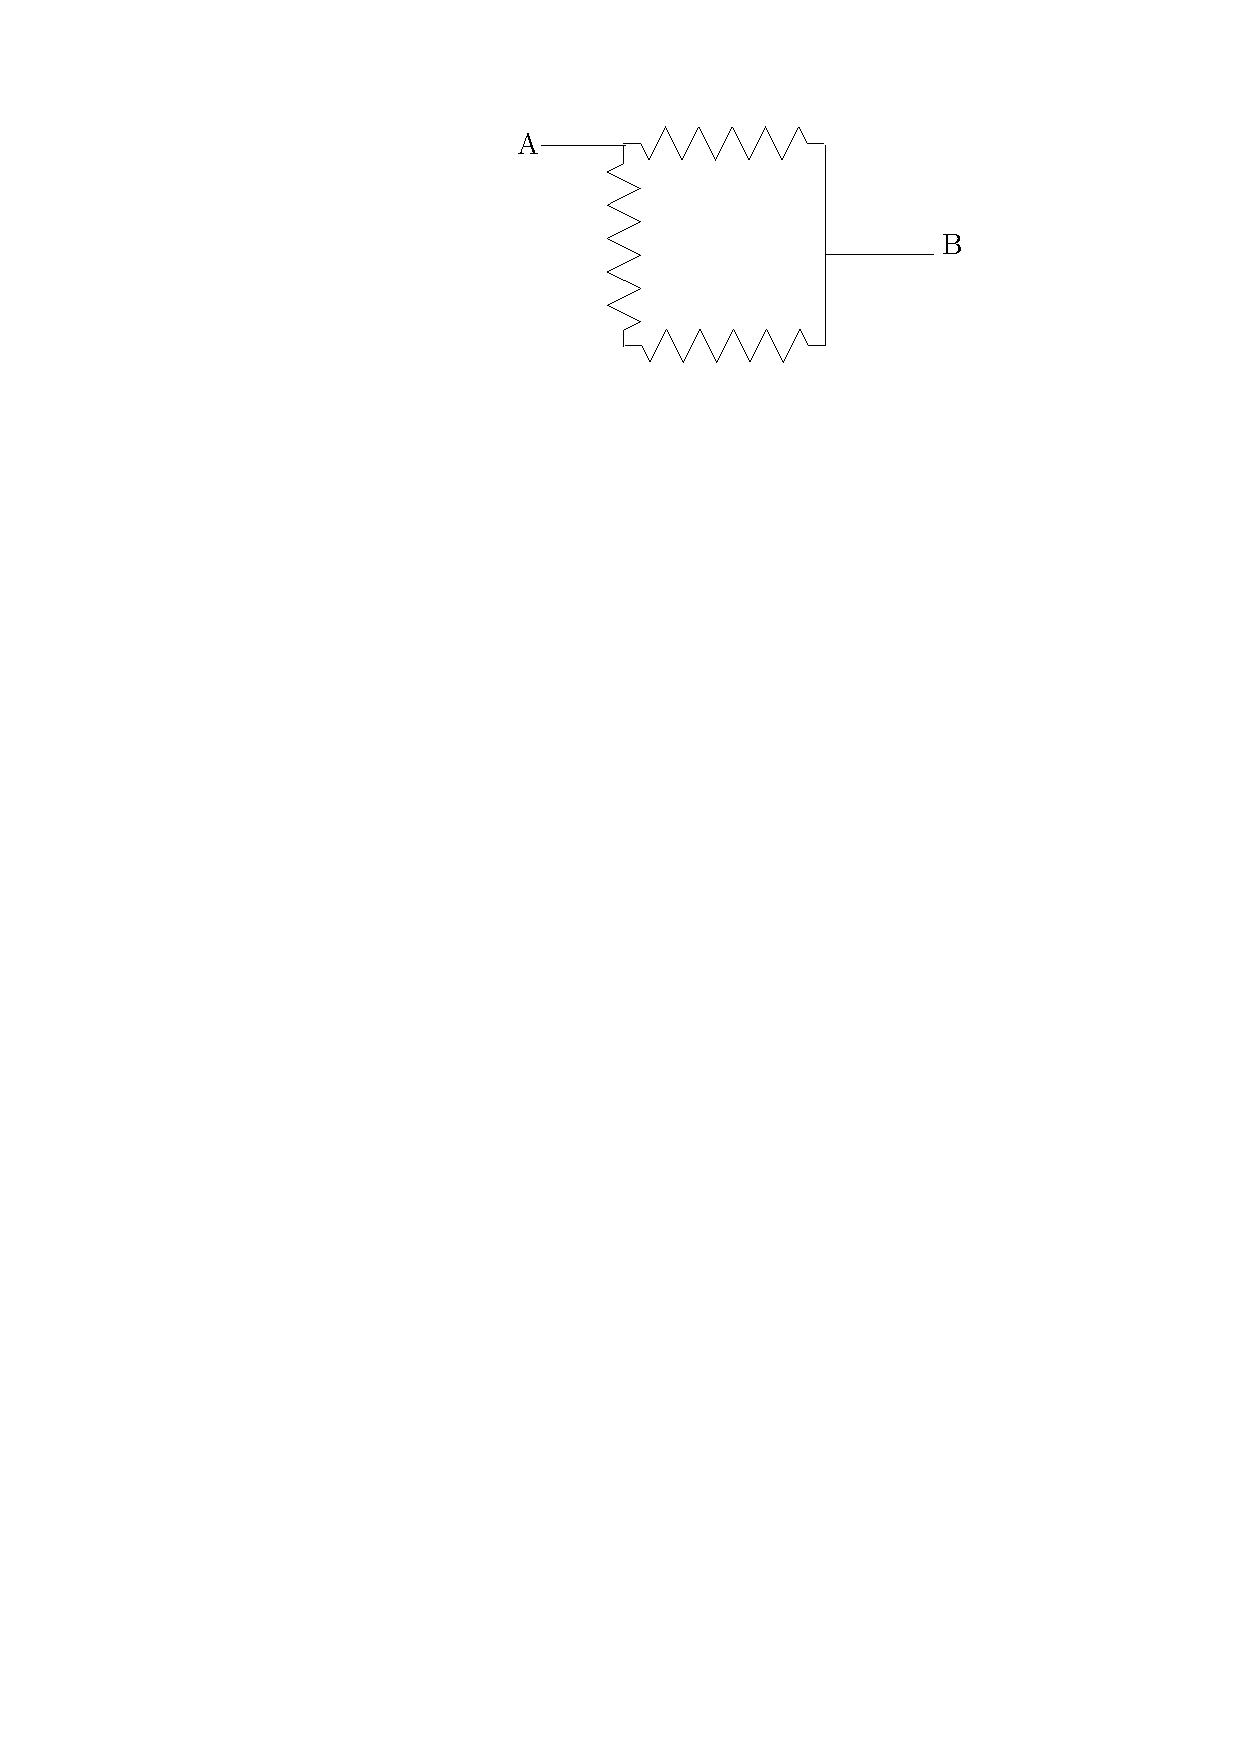
\includegraphics[width=0.35\textwidth]{resistor_series.pdf}

\newpage

\noindent Compute the current and power dissipated through each resistor.  

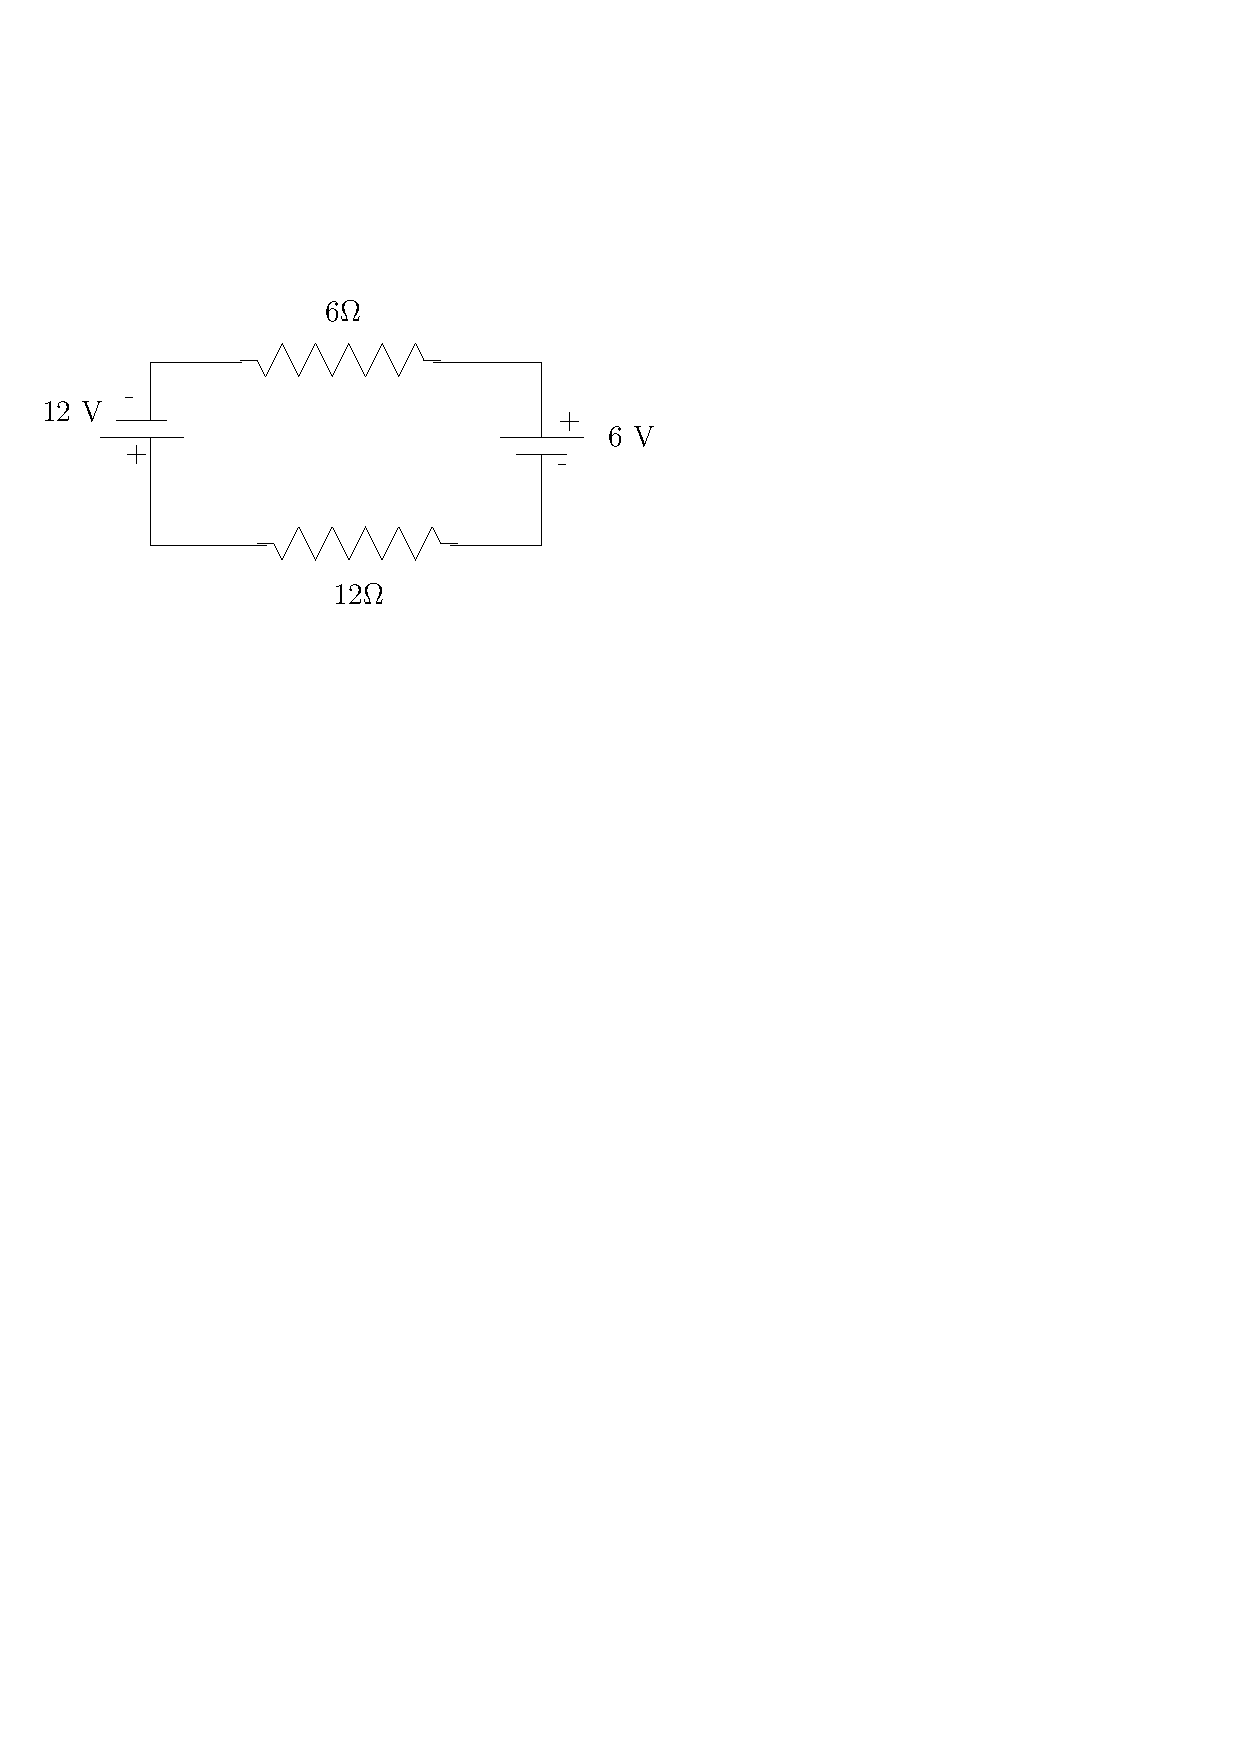
\includegraphics[width=0.4\textwidth]{kirchoff1.pdf}

\newpage 

\noindent Compute the current through each branch of this circuit.  

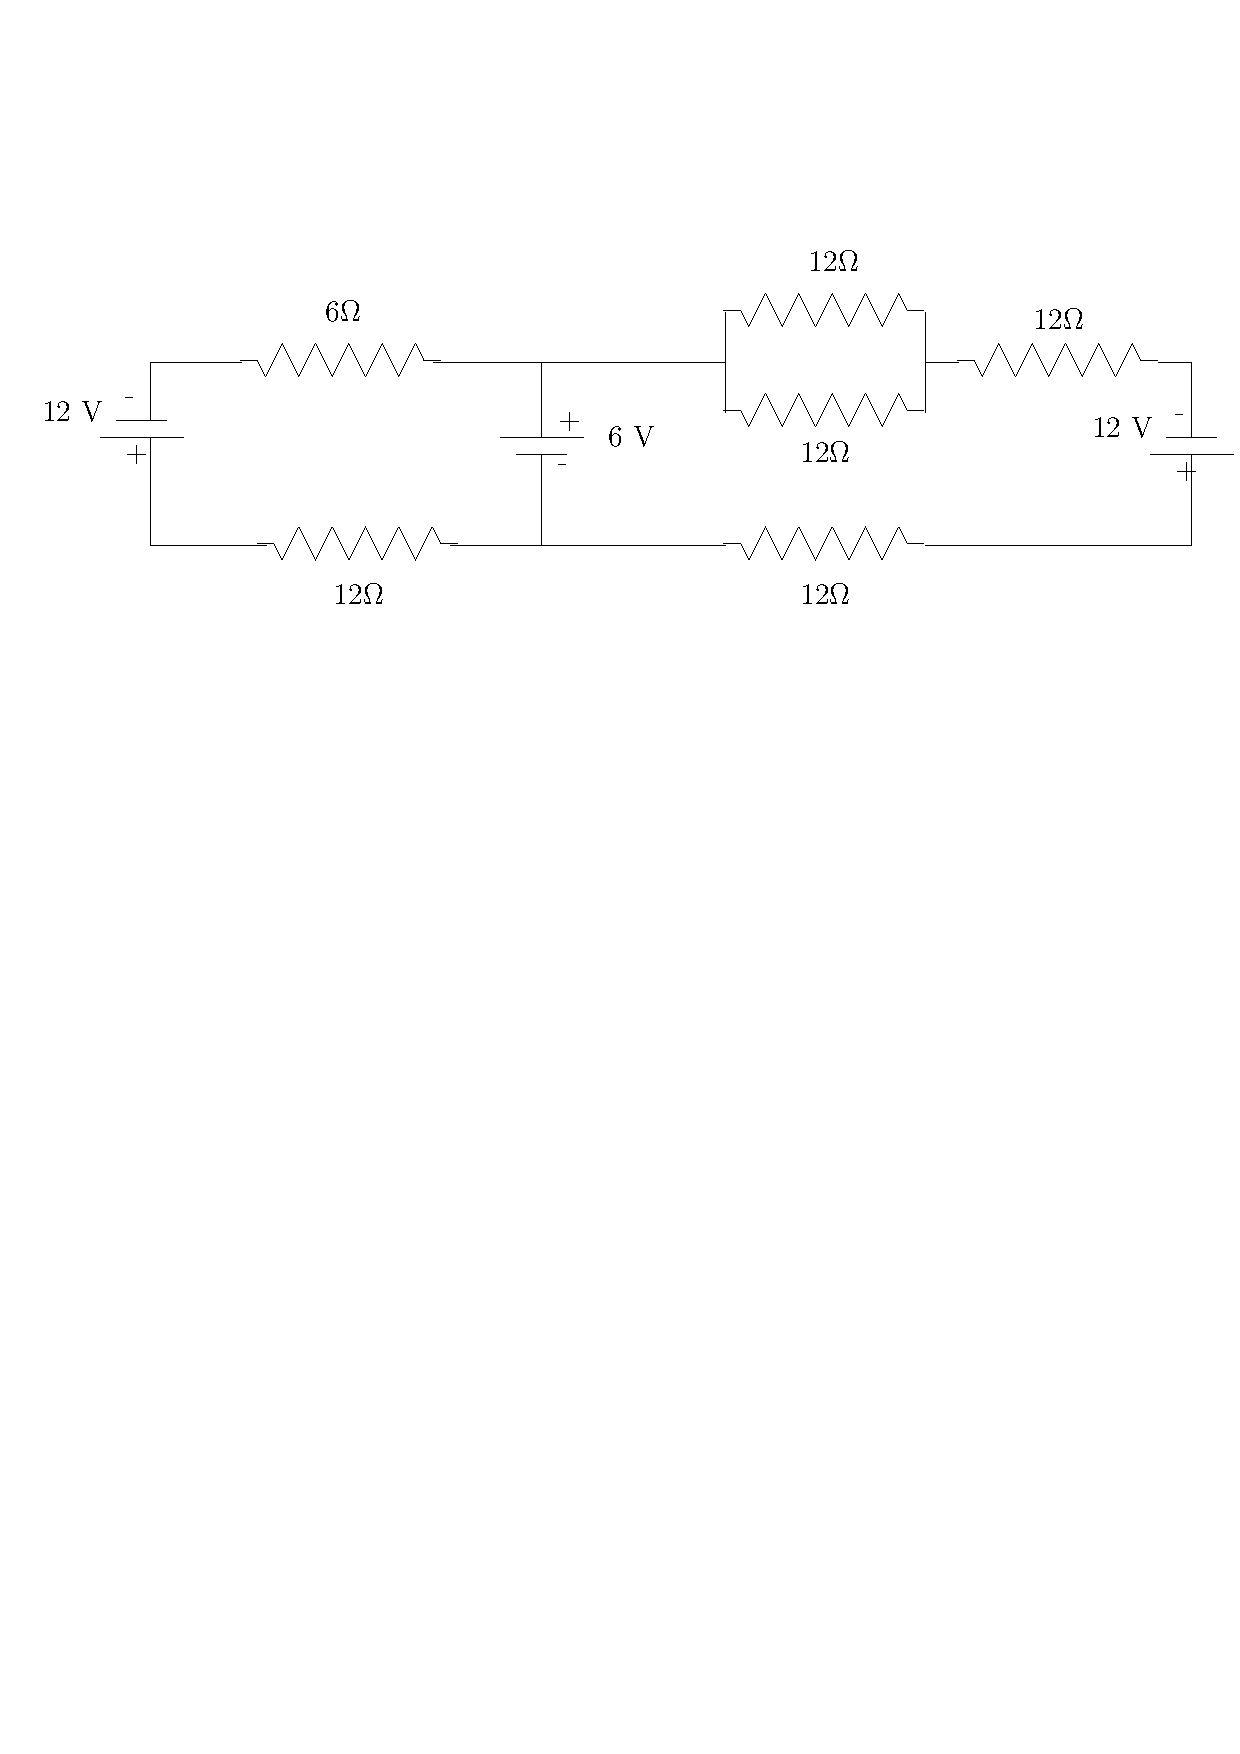
\includegraphics[width=0.7\textwidth]{kirchoff2.pdf}

\newpage

\noindent Consider the following infinite ladder of identical resistors.  Find the equivalent resistance between A and B.  

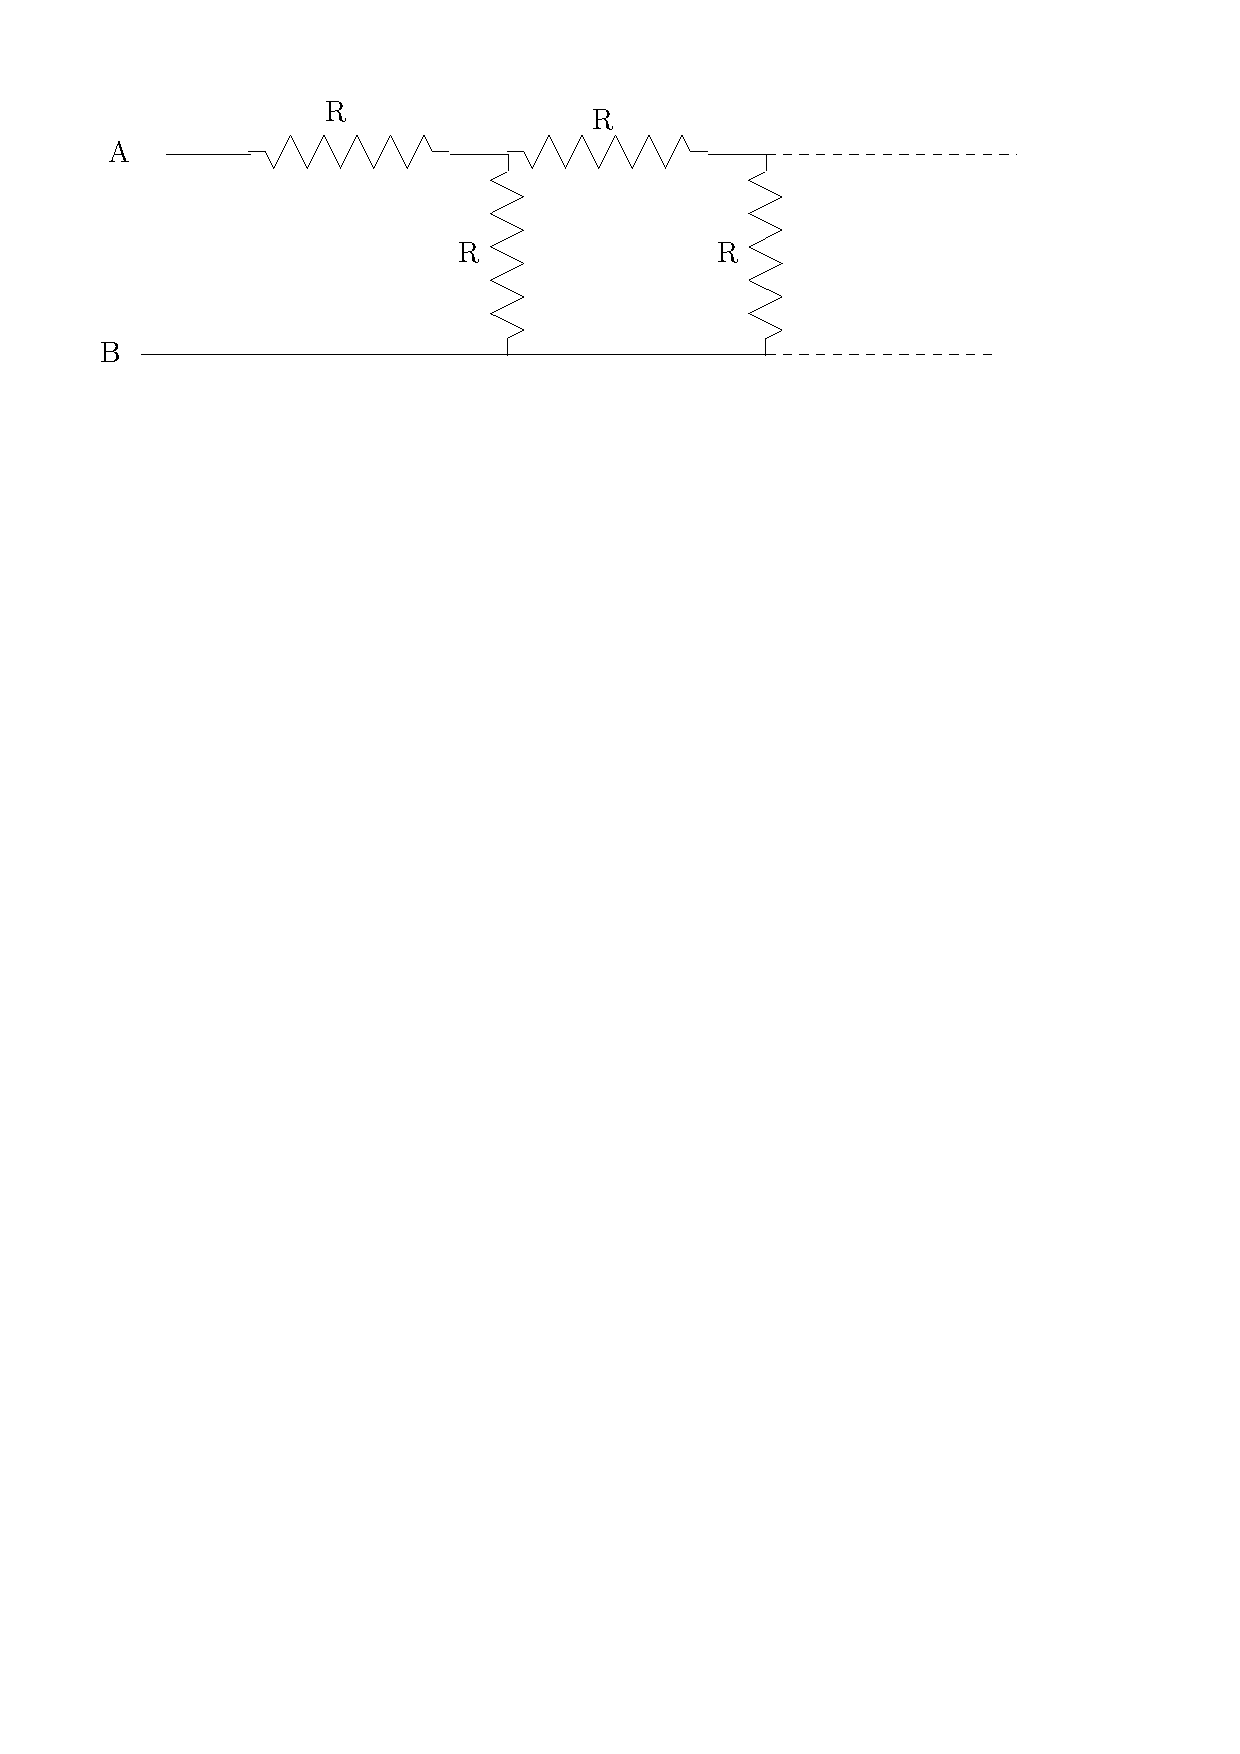
\includegraphics[width=0.6\textwidth]{infinite_ladder.pdf}
\end{document}
